\chapter{Development}\label{ch:C}

\section{iOS}

\subsection{Architecture}

First of all, we built the architecture of the application. For the architecture, we have adopted Service Oriented Architecture (SOA), a software development style that integrates functionality and business logic in such a way that services can be injected into view controllers for use. \textit{(see Figure \ref{fig:ProjectStructure}) }

\begin{figure}[h]
    \centering
    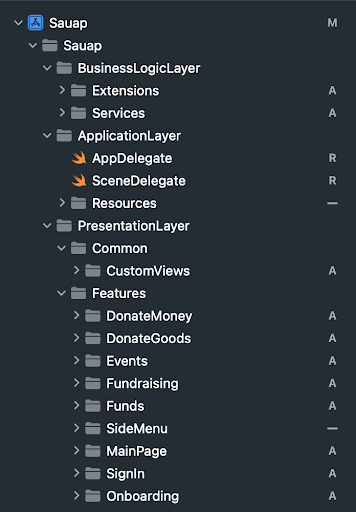
\includegraphics[scale=0.4]{figures/iOS/ios1.png}
    \caption{Project Structure}
    \label{fig:ProjectStructure}
\end{figure}
The project root is divided into 3 folders:

\begin{itemize}
    \item[----] The BusinessLogicLayer contains Services as a manager for API calls and Extensions with extended functionality of existing components. 
    \item[----] ApplicationLayer contains the AppDelegate.swift, SceneDelegate.swift files and the necessary resources.
    \item[----] PresentationLayer contains Features, which contains MVC modules under the features of the application, and Common, which contains the main common components for all modules for reuse.
\end{itemize}

Services allow us to port specific business logic implementations from our UIViewControllers, making them easier to read and maintain.

There are three components in this design pattern: Model, View, and Controller.

\begin{figure}[h]
    \centering
    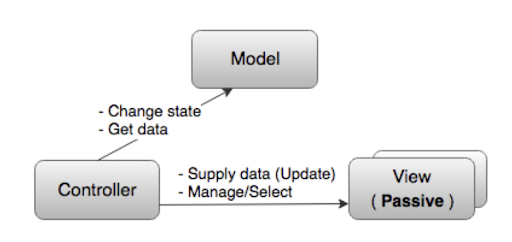
\includegraphics[scale=0.4]{figures/iOS/ios2.png}
    \caption{Visual representation of MVC}
    \label{fig:VisualrepresentationofMVC}
\end{figure}

\begin{itemize}
    \item[----] Model -- the data necessary for the operation of the application and logic, operations on this data.
    \item[----] View -- the visual part of the application, handling user interaction.
    \item[----] Controller -- provides communication between the Model and the View, that is, it receives the user's input and performs some operations or receives data from the network, then updates the View.
\end{itemize}

\begin{figure}[h]
    \centering
    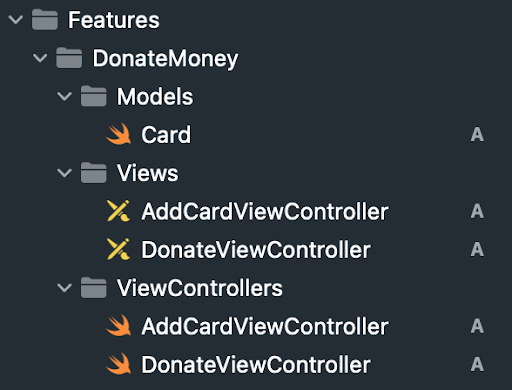
\includegraphics[scale=0.4]{figures/iOS/ios3.png}
    \caption{MVC in our project}
    \label{fig:MVCinourproject}
\end{figure}

\subsection{Dependency Management}

For the Sauap project, we used the dependency manager, CocoaPods, for the Swift and Objective-C Cocoa projects. It helps to scale the project in a convenient way, which provides an optimal way to manage dependencies. Libraries are specified in the Podfile, a file describing the application's dependencies. This file is shown in \textit{Appendix \ref{app:appendixA}}.


Third Party Libraries used in the project:
\begin{itemize}
    \item[----] Firebase - We used server services for native authentication and ready-made interfaces for authorization and storage of authentication data, which you can see in \textit{Appendix \ref{app:appendixB}}:
    \item[----] Alamofire - a library that simplifies network requests.
    \item[----] SDWebImage - used to asynchronously download photos from the network.
\end{itemize}

\subsection{App Navigation}

Navigation in the application is carried out using the side menu. In code, this happens in the ContainerViewController class \textit{(see Figure \ref{fig:ContainerViewController})}, which acts as a parent viewcontroller and adds other viewcontrollers to its hierarchy, which ensures page changes.

Child view controllers are especially useful for user interface features that we want to reuse in a project. For example, the screen from the Fundraising section also has an entry point from the main page, which can be added to the navigation stack of the main page viewcontroller in a very simple way.

\begin{figure}[h]
    \centering
    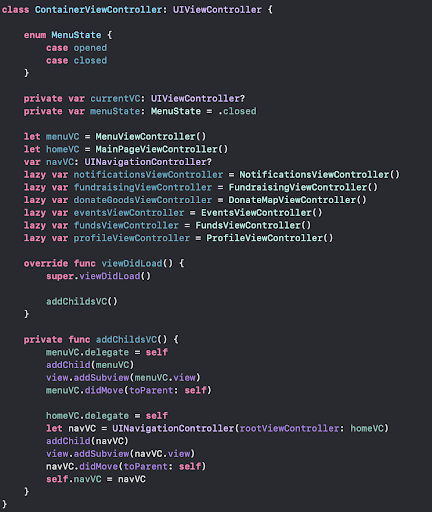
\includegraphics[scale=0.45]{figures/iOS/ios4.png}
    \caption{ContainerViewController.swift}
    \label{fig:ContainerViewController}
\end{figure}

\section{Backend}

    All the logic of the main functionality is implemented in the server part. The data is separated from the logic of the applications and is stored in the storage. For example, there is a section with funds on the applications, then there is exactly one handler for displaying the list of funds, which the front application sends data to the back via the REST API, and the data is stored in the database and will be received using the back applications.

    One of the server programming languages is used to describe application logic. Theoretically, almost any language \cite{golang} can be used to create applications, but as it happens, we use Java as the main programming language for the backend part
    
    The main way of development is a framework. It provides ready-made solutions for typical tasks, such as working with Rest APIs, integration with databases, technologies, and much more. Spring Boot is the main framework of our back service
    
    The main task of the back service was to make a REST API for working with data by implementing application logic where the front application could integrate. We have divided the logic of the work into several parts:
    \begin{itemize}
        \item Endpoints for working with users 
        \item Endpoints for working with funds
        \item Endpoints for working with fundraise
        \item Endpoints for working with collection points
    \end{itemize}
    
    As a result, all the endpoints were displayed in Swagger-UI
    
    \begin{figure}[h]
        \centering
        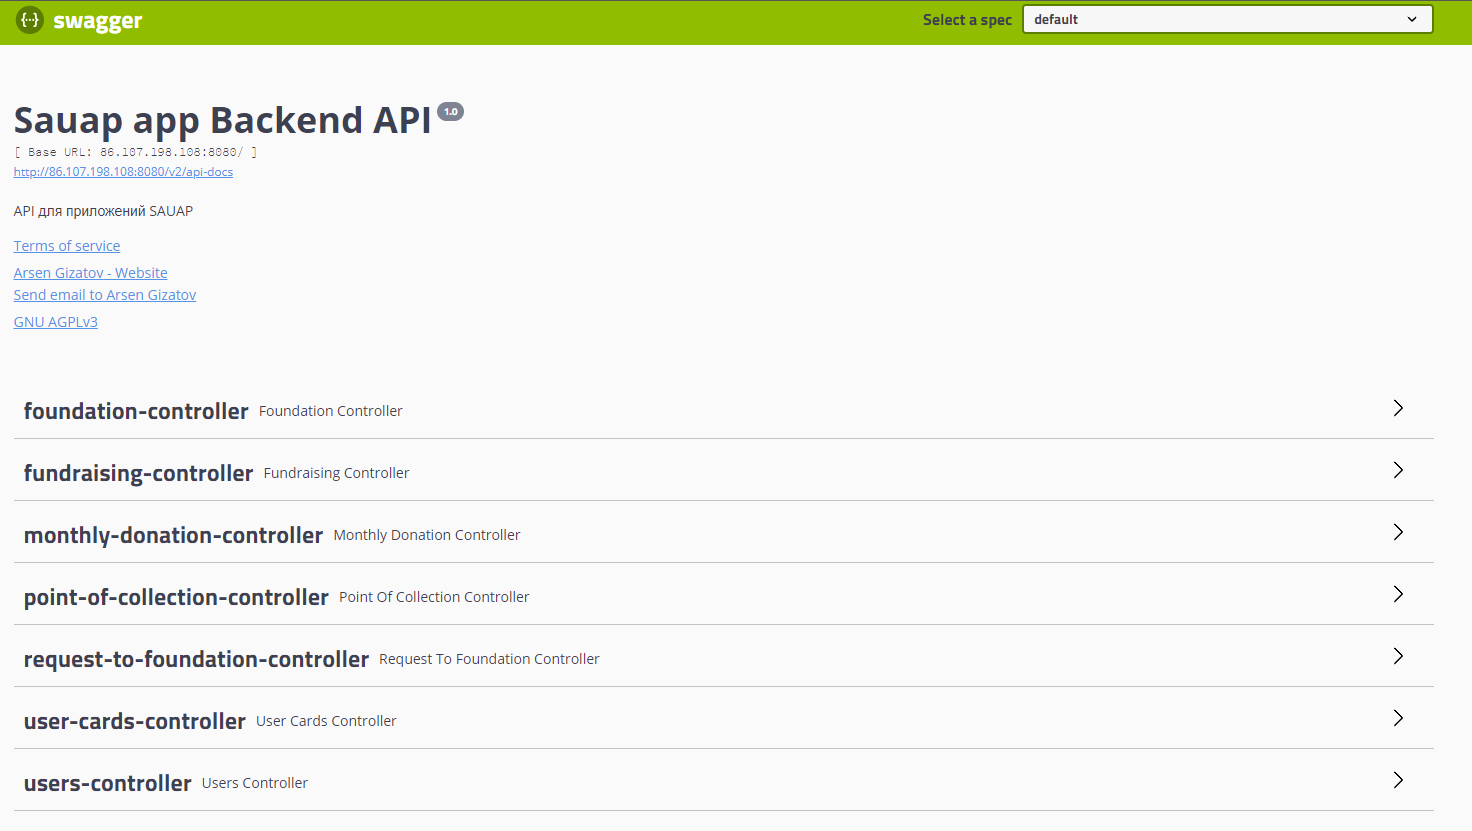
\includegraphics[width=13cm]{figures/swagger.png}
        \caption{Swagger-UI page (details about API)}
        \label{fig:13}
    \end{figure}
    
    The service has logic for working with mail and payments and with Amazon WS services, more precisely Amazon S3 for working with file system distributors. We use this system to store data in a large volume such as files, photos, videos, etc. 
    
\subsection{Data Storage}
    
    We used a PostgreSql database as a data storage. PostgreSql is not just a relational, but an object-relational DBMS, as well as one of the fastest and most functional databases. To implement the logic of the application, it was first necessary to build the architecture of the system. The architecture has normalization and basically one-to-many relationships.
    
    \begin{figure}[h]
        \centering
        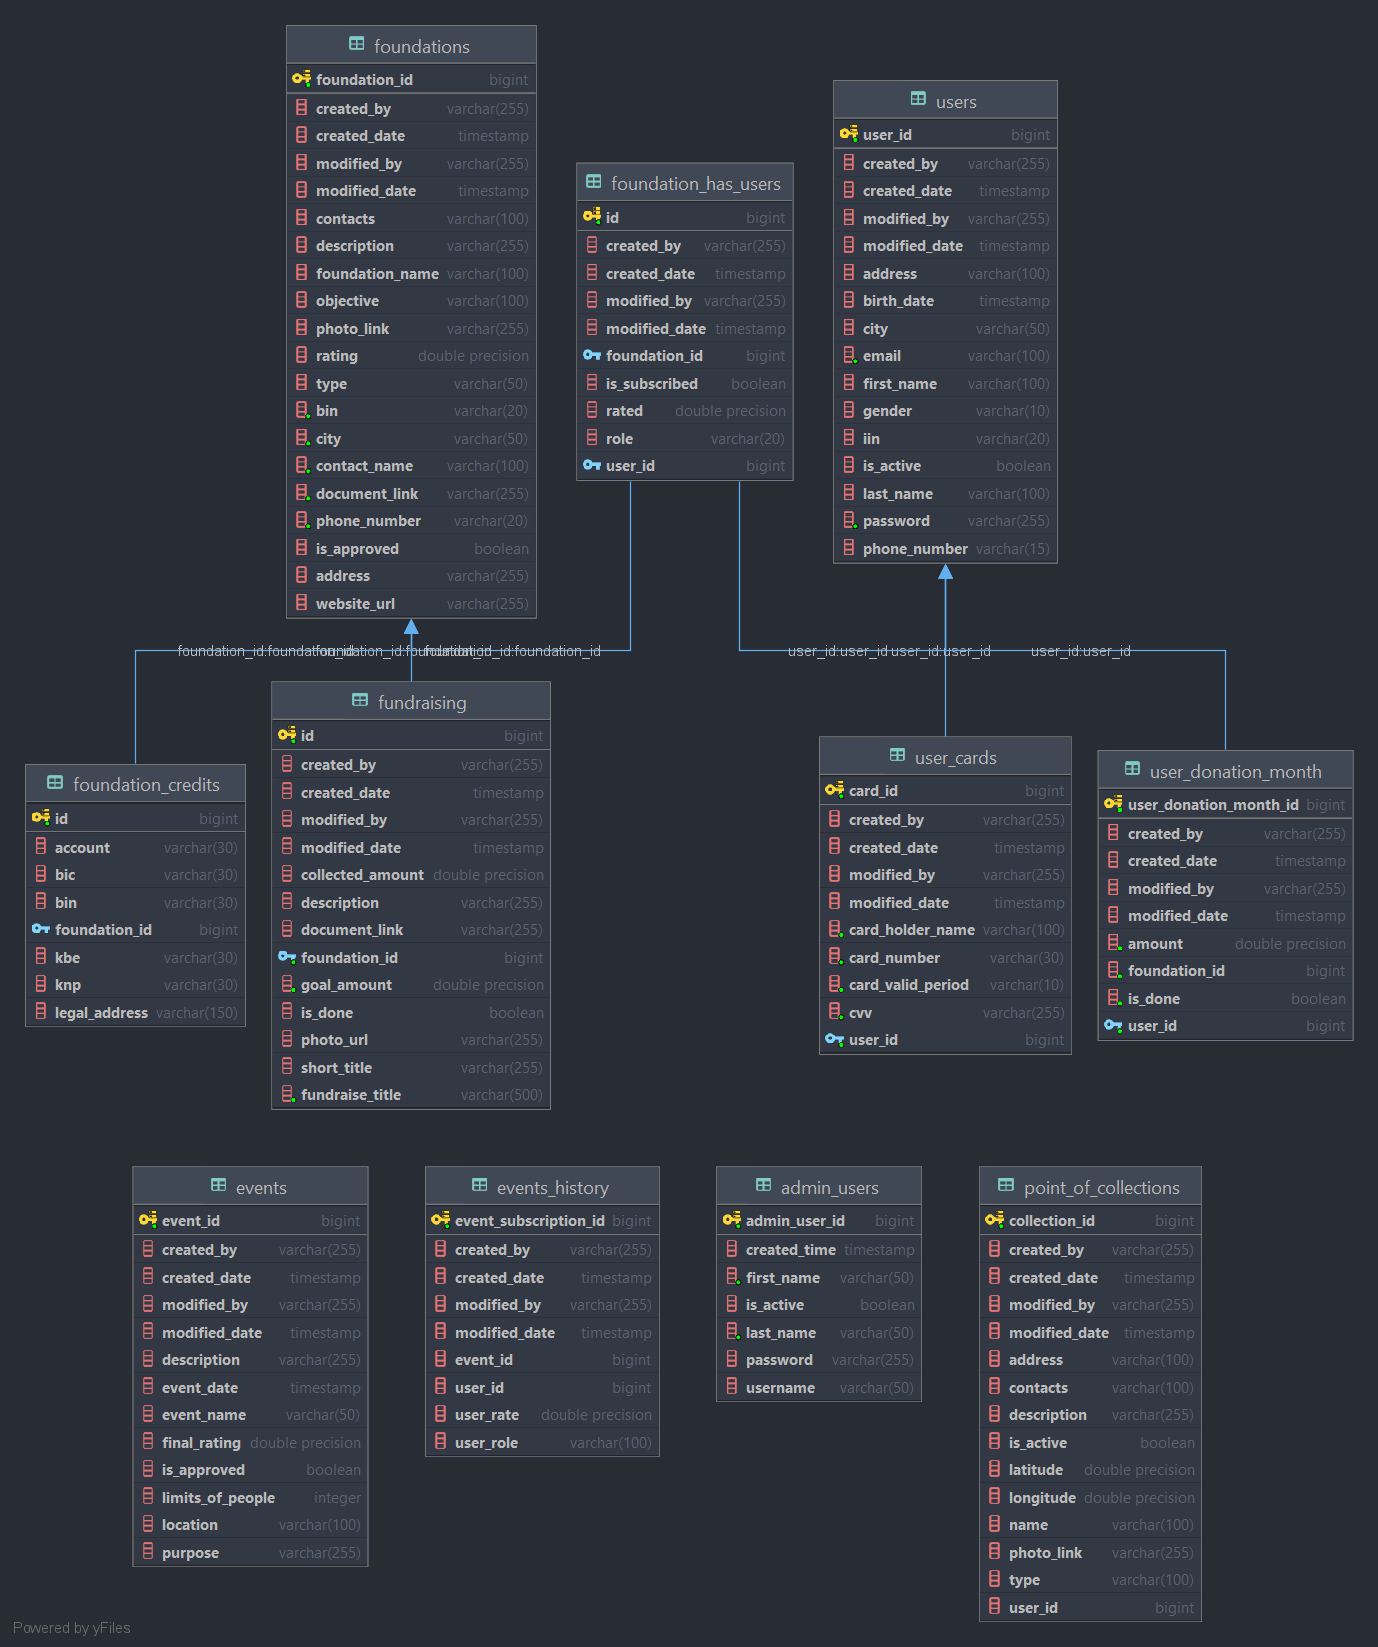
\includegraphics[width=13cm]{figures/uml.png}
        \caption{UML-diagram}
        \label{fig:Uml diagram}
    \end{figure}

\subsection{Admin UI}

To create the admin panel, we used a tool called Retool \cite{Retool}, which helps us connect our database, in our case Endpoint, and display them on a specific page. With it, we do CRUD operations. That is, it is Creating, Adding, Updating and Deleting data to our database. The admin panel will be used directly by employees of various foundations to manage all the processes that will occur directly with their organization in our application.

And to write Endpoints, we used Java code \cite{Java}, and raised it through Swagger so that we could use it for further settings.


\begin{figure}[h]
    \centering
    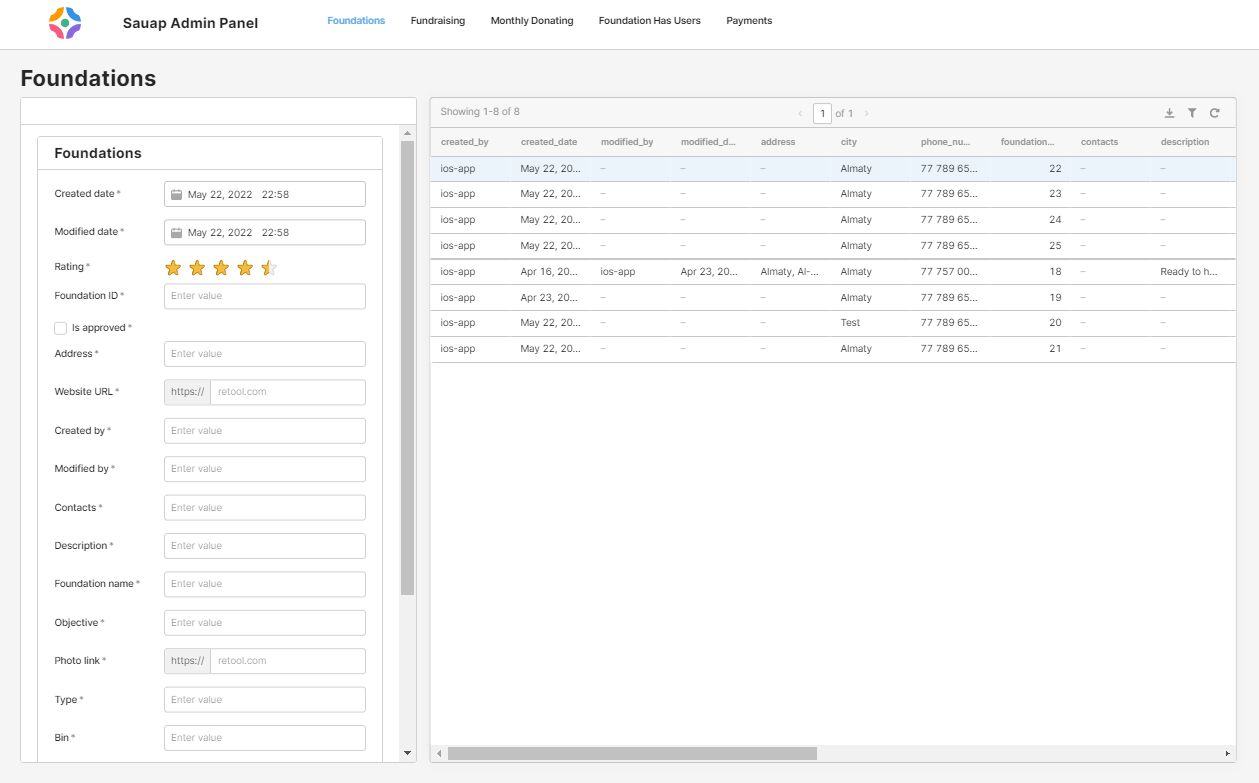
\includegraphics[width=13cm]{figures/adminPanel.png}
    \caption{Admin panel}
    \label{fig:14}
\end{figure}

